\chapter{Documento di design}
In questa sezione vengono illustrate le scelte architetturali e i design pattern adottati nel software.
Un design pattern è una soluzione generale e collaudata per risolvere problemi ricorrenti che si incontrano durante la progettazione di software.
Questi pattern possono migliorare la comprensione del codice, la manutenzione e la scalabilità di un'applicazione.

\bigskip\bigskip

\section{Architettura del Software}
L'architettura del software è suddivisa tra il client e il server, con il client sviluppato in Flutter e il server utilizzando AWS.

\subsection{Client}
L'applicazione client è sviluppata utilizzando Flutter, un framework open-source di Google per la creazione di applicazioni mobili nativamente compilate. Flutter consente di creare un'interfaccia utente ricca e reattiva, mantenendo un'alta performance sia su Android che iOS.\meskip
Il client sarà responsabile della visualizzazione dei dati e dell'interazione con l'utente.\\
La gestione dello stato sarà gestito tramite il pattern MVC (Model-View-Controller) integrato con i DAO (Data Access Object).
Questo approccio separa la logica di business, la gestione dello stato e l'accesso ai dati, migliorando la manutenibilità e la testabilità del codice.

\subsection{Server}
Per la gestione del server, abbiamo scelto Amazon Web Services (AWS), una piattaforma cloud che offre un'ampia gamma di servizi, tra cui elaborazione, archiviazione, e database.
Il server è stato implementato utilizzando un'istanza EC2, con un database gestito tramite RDS e la logica applicativa eseguita su un backend sviluppato in Express.


\subsection{Interazione tra Client e Server}
Il client invia richieste HTTP al backend seguento l'architettura REST. Il server riceve queste richieste, le elabora, e interagisce con il database per ottenere o aggiornare i dati.

Le risposte vengono restituite al client in formato JSON, garantendo così una facile integrazione e manipolazione dei dati all'interno dell'applicazione Flutter.

La comunicazione tra client e server avviene attraverso richieste asincrone, che permettono al client di ottenere dati aggiornati in tempo reale senza interrompere l'esperienza dell'utente.

\section{Design pattern utilizzati}

\subsection{Model-View-Controller (MVVM)}
Il pattern Model-View-ViewModel (MVVM) è stato scelto per strutturare l'applicazione in modo da separare le responsabilità e facilitare la manutenzione del codice.

\begin{itemize}
	\item \textbf{Model}: Gestisce i dati dell'applicazione ed è responsabile della notifica alla View quando i dati cambiano. Questo permette alla View di aggiornarsi e riflettere le modifiche senza dover essere a conoscenza dei dettagli di come i dati sono gestiti.

	\item \textbf{View}: Si occupa della presentazione e dell'interfaccia utente. Mostra i dati agli utenti e aggiorna la visualizzazione in risposta alle modifiche del Model.

	\item \textbf{ViewModel}: Funziona da intermediario tra il Model e la View. Gestisce gli input degli utenti e aggiorna il Model e la View di conseguenza.
\end{itemize}

\subsection*{Vantaggi Principali}
\begin{itemize}
    \item \textbf{Separation of Concerns}: Il pattern MVVM promuove una chiara separazione tra la logica di business, la logica di presentazione e l'interfaccia utente, facilitando la manutenzione e l'espansione del codice.
    
    \item \textbf{Testabilità}: La logica dell'applicazione è centralizzata nel ViewModel, che può essere facilmente testato indipendentemente dalla View, rendendo più semplice lo sviluppo di test unitari.
    
    \item \textbf{Data Binding}: MVVM sfrutta il data binding bidirezionale, permettendo di aggiornare automaticamente l'interfaccia utente quando i dati nel ViewModel cambiano, migliorando l'esperienza utente e riducendo il codice boilerplate.
    
    \item \textbf{Modularità}: La separazione tra View e ViewModel consente di riutilizzare componenti e logica in diverse parti dell'applicazione senza duplicazione del codice.
\end{itemize}


\section{Analisi delle scelte tecnologiche utilizzate}
\subsection{Client: Confronto con altre tecnologie}
La decisione di utilizzare flutter è stata presa dopo un'analisi delle opzioni disponibili, considerando vari fattori come la produttività, le prestazioni e la compatibilità.

\subsubsection{React Native}
\begin{itemize}
	\item \textbf{Prestazioni:} Flutter compila il codice direttamente in codice nativo, mentre React Native utilizza un ponte per comunicare tra JavaScript e codice nativo. Questo può portare a prestazioni superiori in Flutter.
	\item \textbf{Coerenza dell'UI:} Flutter utilizza un motore di rendering proprietario, che garantisce una coerenza visiva su tutte le piattaforme, mentre React Native si basa sui componenti nativi, il che può comportare variazioni tra iOS e Android.
\end{itemize}

\subsubsection{Sviluppo nativo (Java/Kotlin per Android, Swift per iOS)}
\begin{itemize}
	\item \textbf{Cross-Platform:} Flutter consente di scrivere un solo codice per entrambe le piattaforme, riducendo i tempi e i costi di sviluppo rispetto alla scrittura di codice separato.
	\item \textbf{Consistenza dell'Interfaccia:} Flutter offre un controllo totale sul rendering e sulla consistenza dell'interfaccia su entrambe le piattaforme.
	\item \textbf{Aggiornamenti e Manutenzione:} La manutenzione di una singola codebase è generalmente più semplice e meno costosa.
\end{itemize}

\subsection{Server}
\subsubsection{Amazon EC2}
\textit{Amazon Elastic Compute Cloud} (EC2) è il servizio di AWS che fornisce capacità di calcolo nel cloud.
Tramite EC2, è possibile eseguire istanze di macchine virtuali configurabili in base alle esigenze del progetto, garantendo flessibilità e controllo totale sull'infrastruttura server.

Nel nostro caso, abbiamo implementato un server \textit{NodeJS} che esegue un backend \textit{express}.

\subsubsection{Amazon RDS}
\textit{Amazon Relational Database Service} (RDS) è il servizio gestito di AWS per database relazionali, che semplifica le attività di configurazione, gestione e scalabilità dei database.

Nel nostro caso, abbiamo impiegato RDS con un database PostgreSQL.

\subsubsection{Express.js}
\textit{Express.js} è un framework per applicazioni web Node.js, utilizzato per sviluppare la logica applicativa del nostro backend. Ci ha permesso di implementare un'API RESTful in modo rapido ed efficiente, gestendo le richieste tra il client e il server e interfacciandosi con il database ospitato su RDS.

\pagebreak

\section{Diagrammi UML di Design}
Di seguito illustriamo i diagrammi UML di Design del sistema.
\subsection{View}
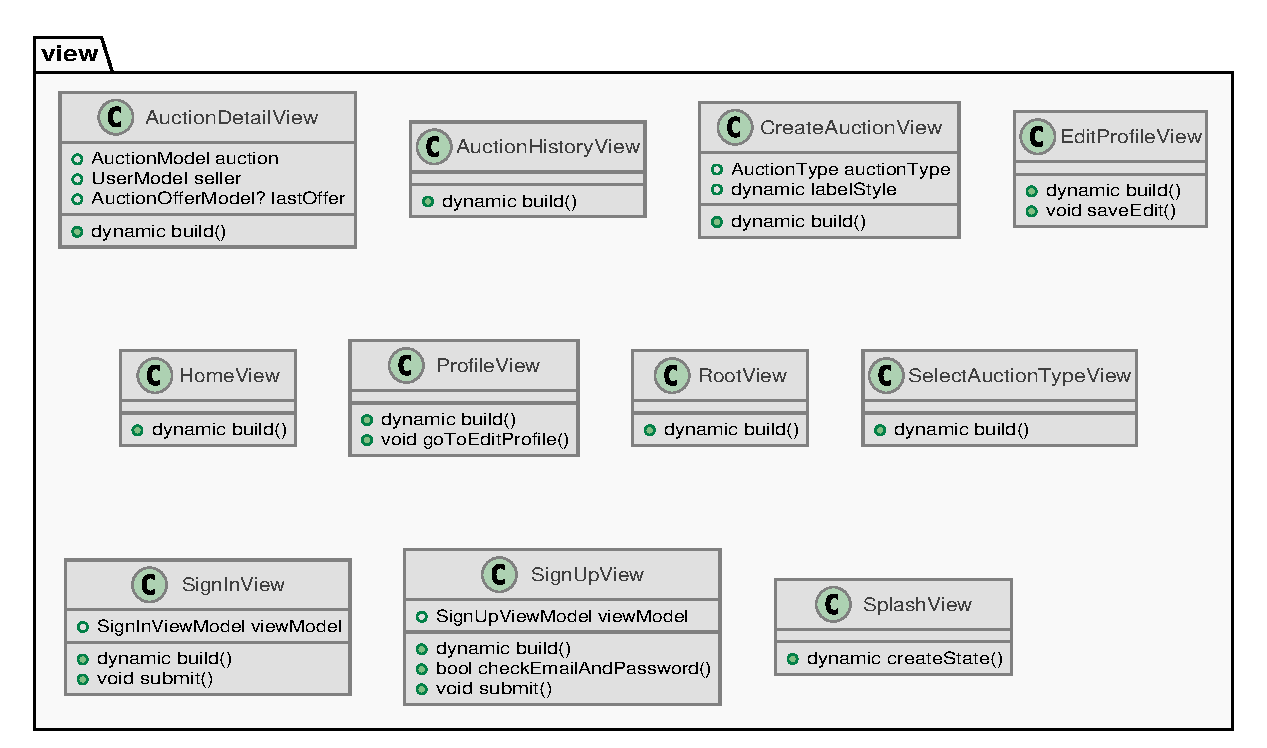
\includegraphics[width=\textwidth]{assets/uml_design/view.pdf}
\subsection{Model}
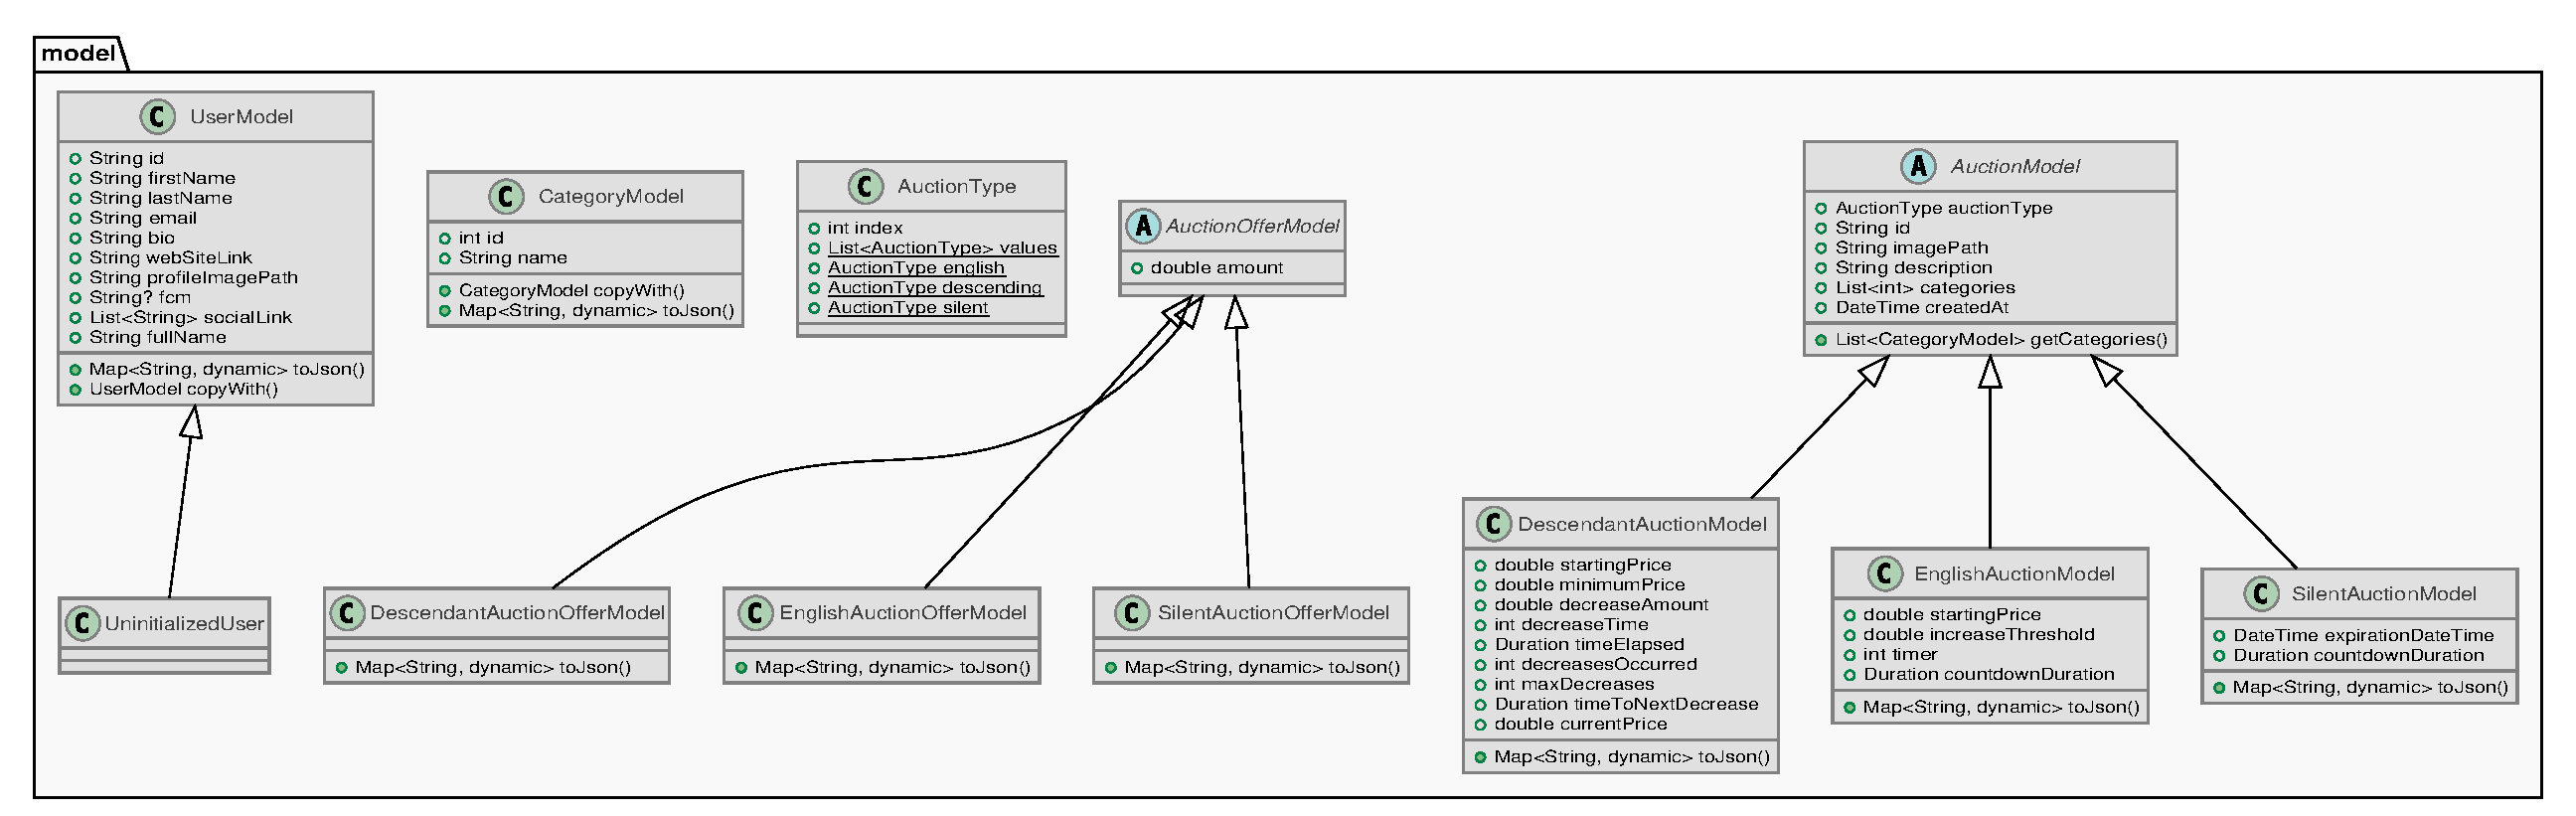
\includegraphics[width=\textwidth]{assets/uml_design/model.pdf}
\subsection{ViewModel}
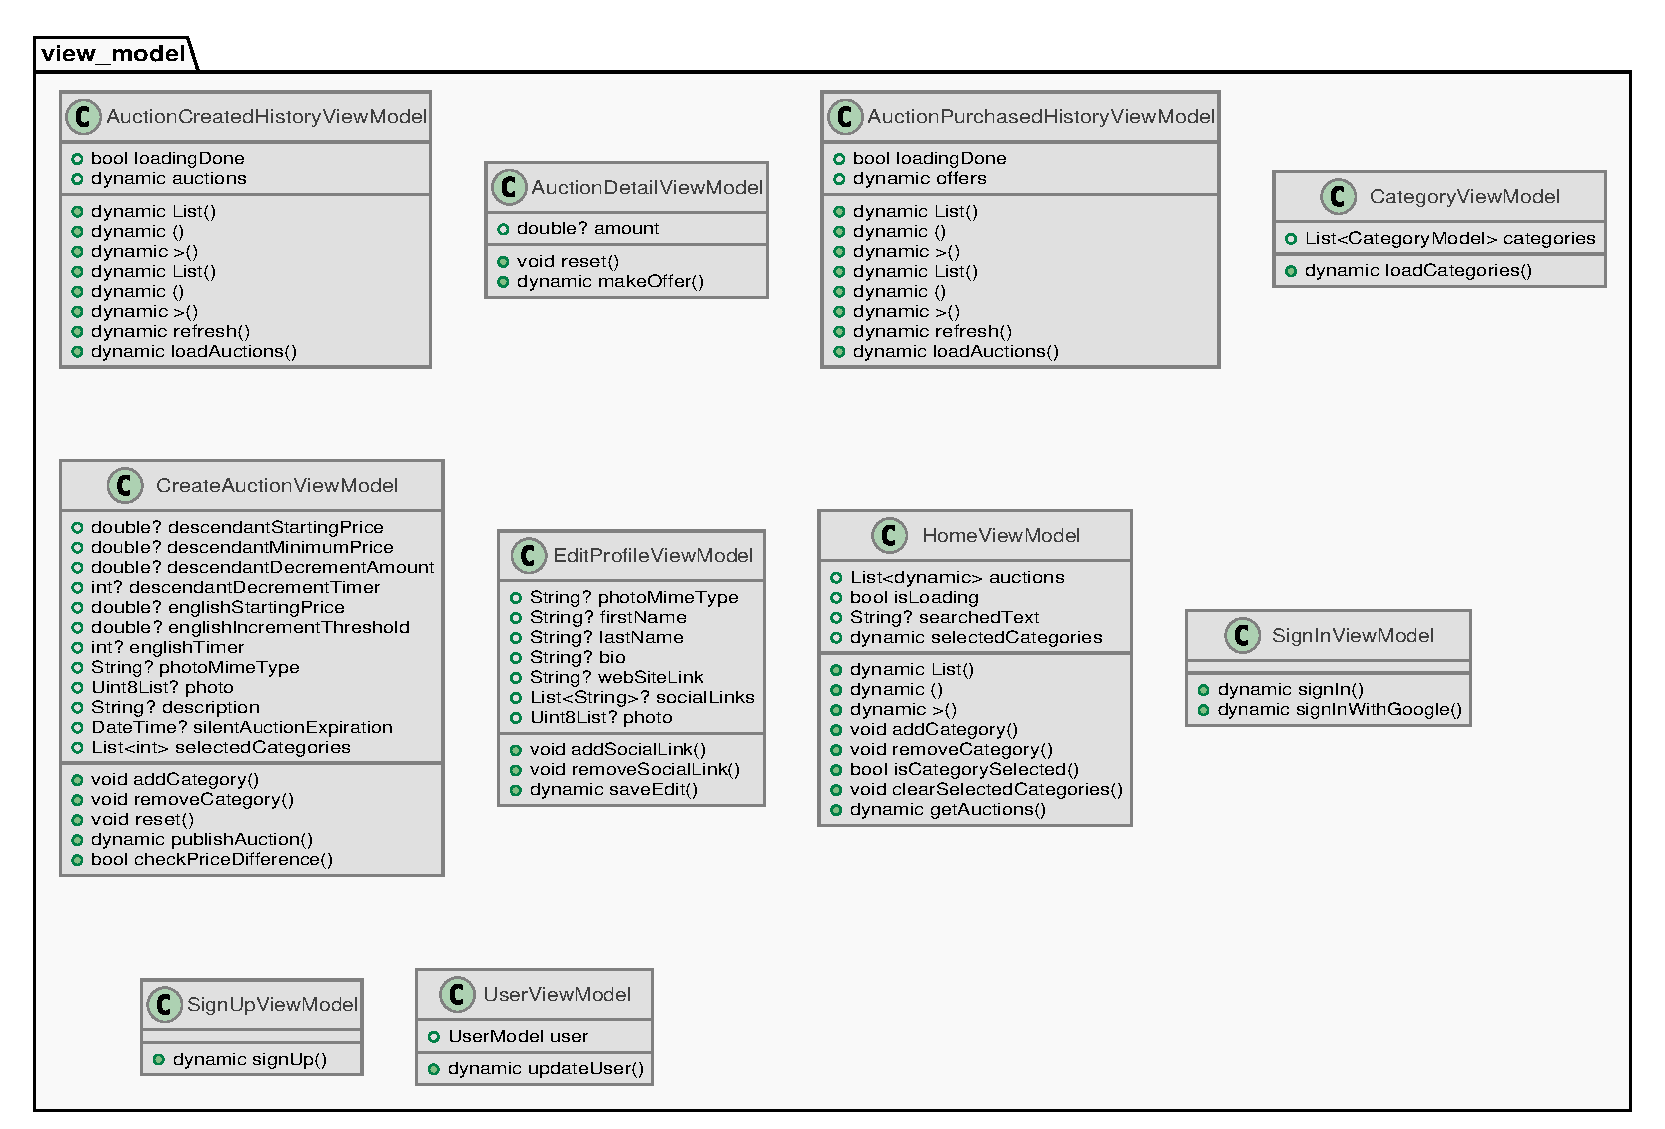
\includegraphics[width=\textwidth]{assets/uml_design/view_model.pdf}
\subsection{Routes}
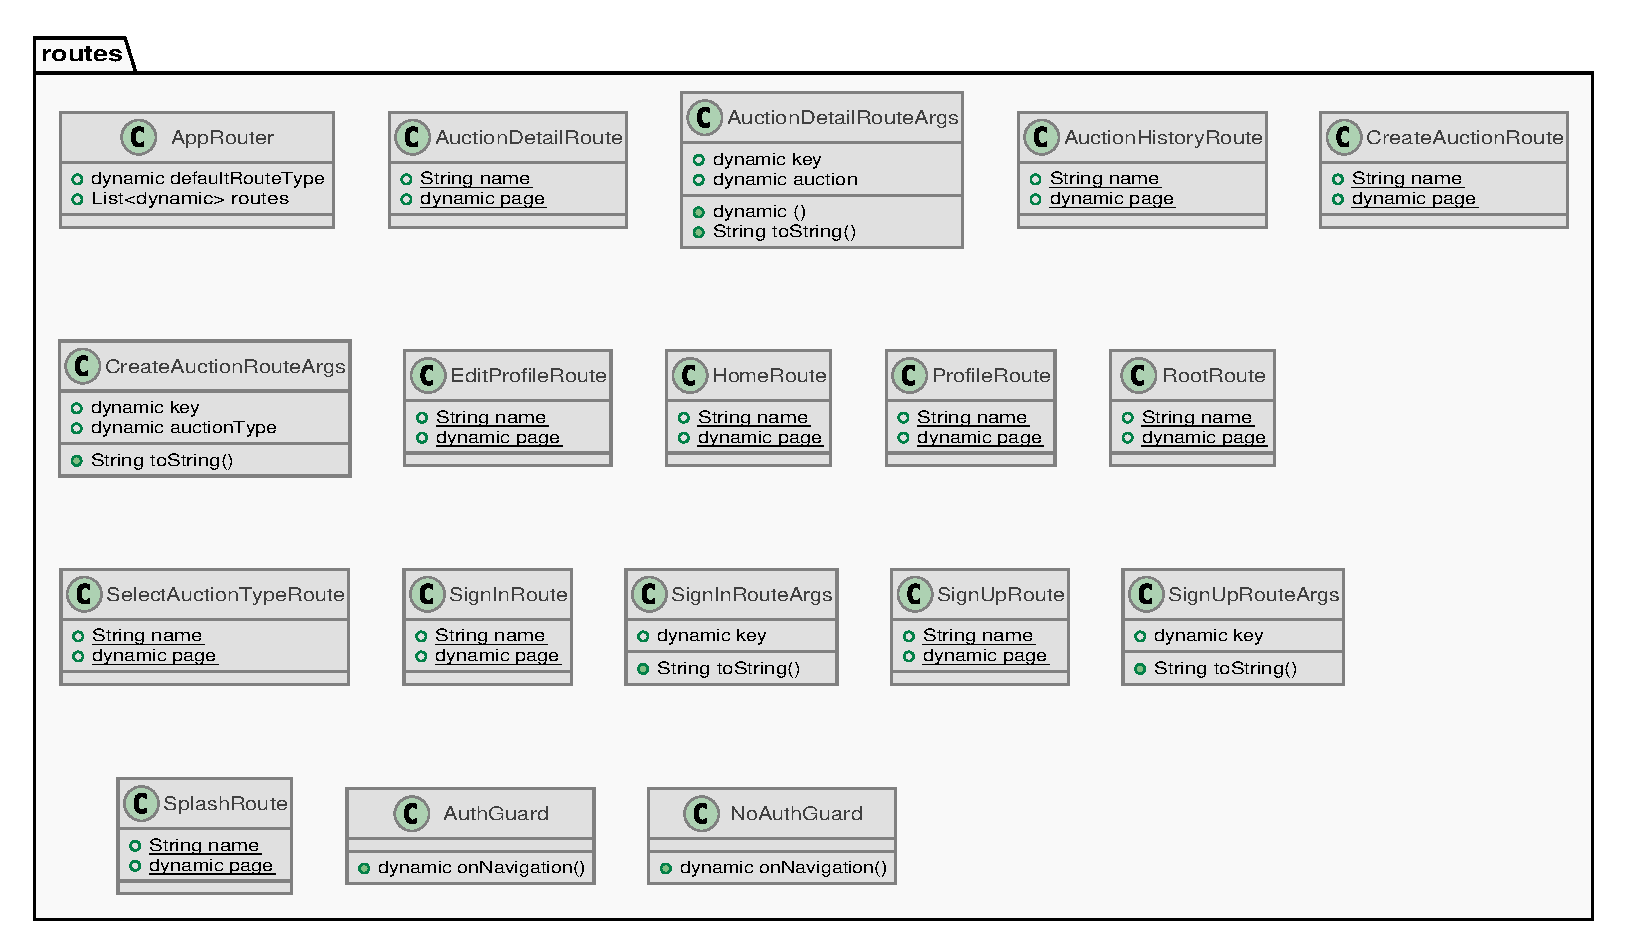
\includegraphics[width=\textwidth]{assets/uml_design/routes.pdf}
\subsection{Services}
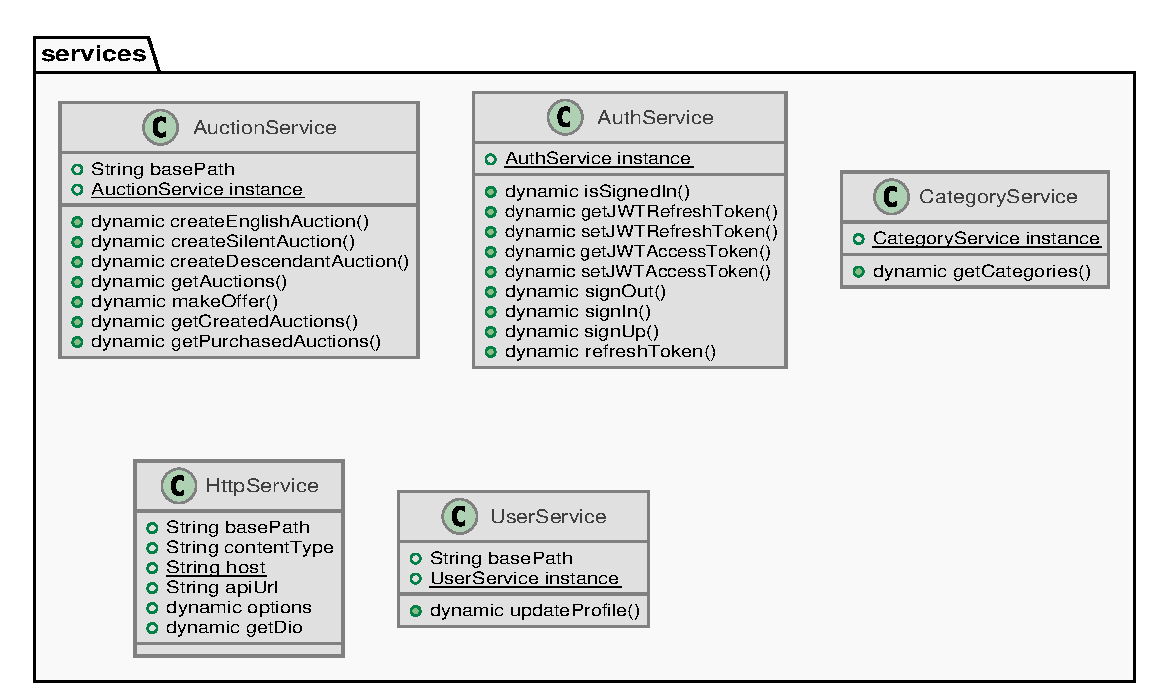
\includegraphics[width=\textwidth]{assets/uml_design/services.pdf}




\section{Diagrammi di Sequenza di Design}
\subsection{Caso d'uso: Creazione Asta Silenziosa}
Il seguente Sequence Diagram descrive il processo di creazione di un'Asta Silenziosa. \\
L'attore principale è l'utente venditore, che compila il form. Il sistema elabora i dati e invia una richiesta al server. \\
Se la richiesta di creazione è andata a buon fine, il sistema si aggiorna correttamente, mantenendo cosi la coerenza con il server esterno, e restituisce un messaggio all'utente mediante l'interfaccia grafica.
Altrimenti, elabora il messaggio di errore ricevuto dal server e restituisce il messaggio d'errore corrispondente all'utente. \bskip
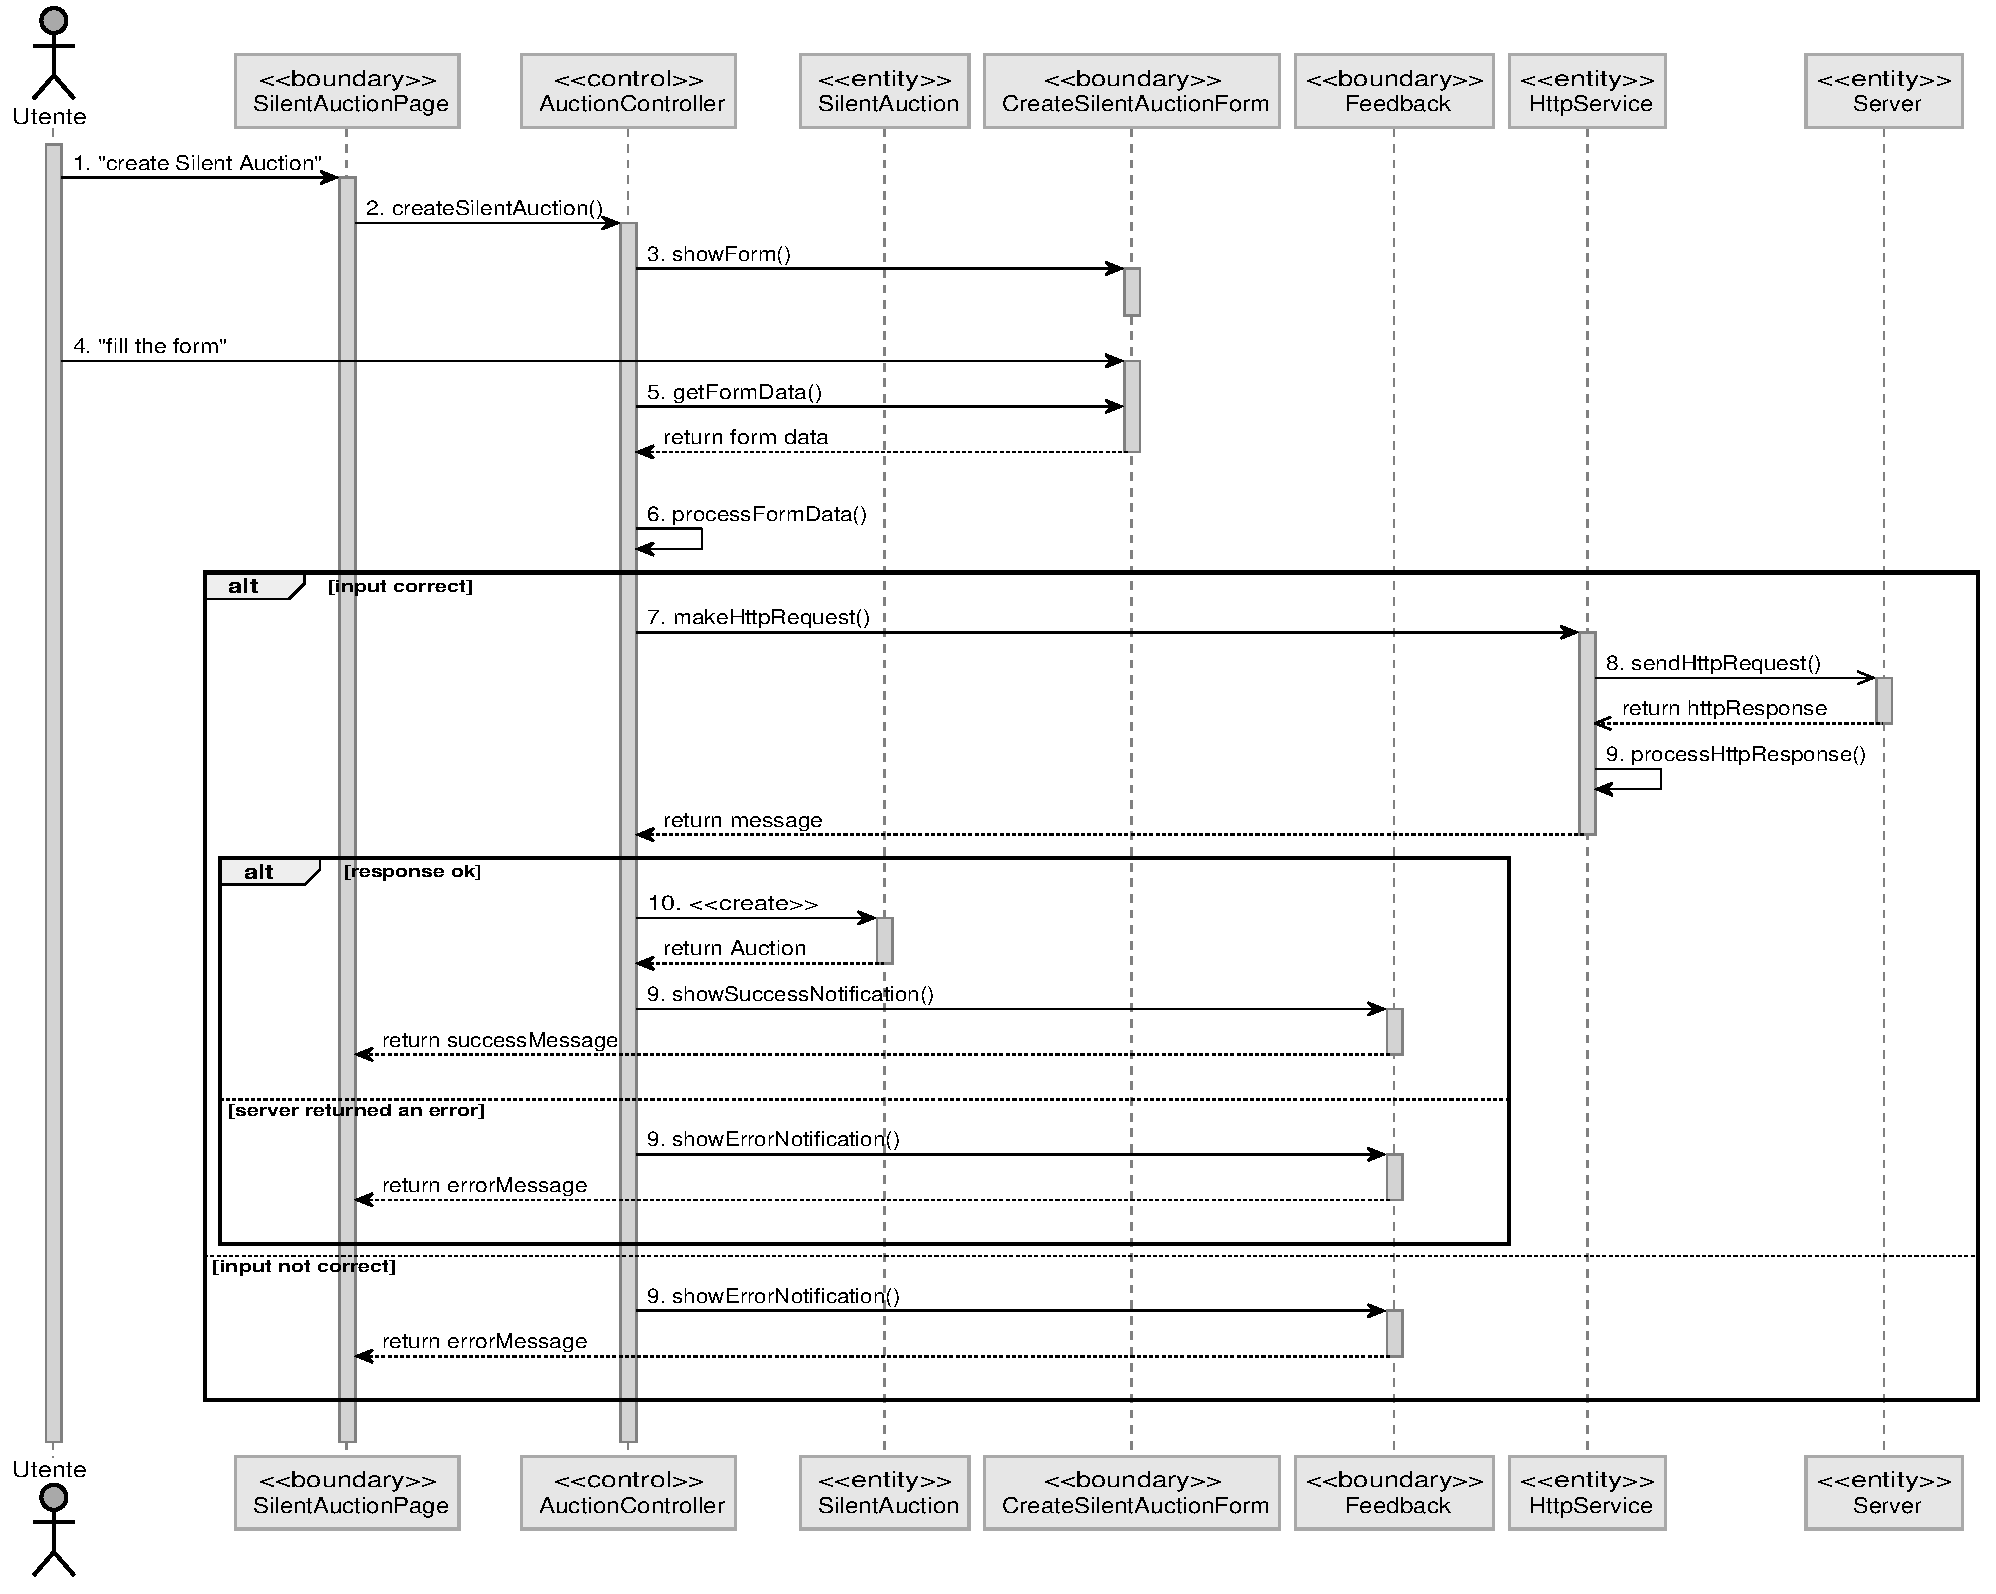
\includegraphics[width=\textwidth]{assets/sequence/creazione_asta_silenziosa.pdf}

\pagebreak
\subsection{Caso d'uso: Offerta Asta Silenziosa}
Il seguente Sequence Diagram descrive il processo di creazione di un'offerta per l'Asta Silenziosa.\\
L'attore principale è l'utente acquirente, che inserisce i dati necessari alla creazione dell'offerta, compilando il form, e invia i dati al sistema.\\
Il sistema verifica che l'asta sia attiva, e invia una richiesta al server per la creazione dell'offerta, restituendo l'esito all'utente, mediante l'interfaccia grafica.\bskip
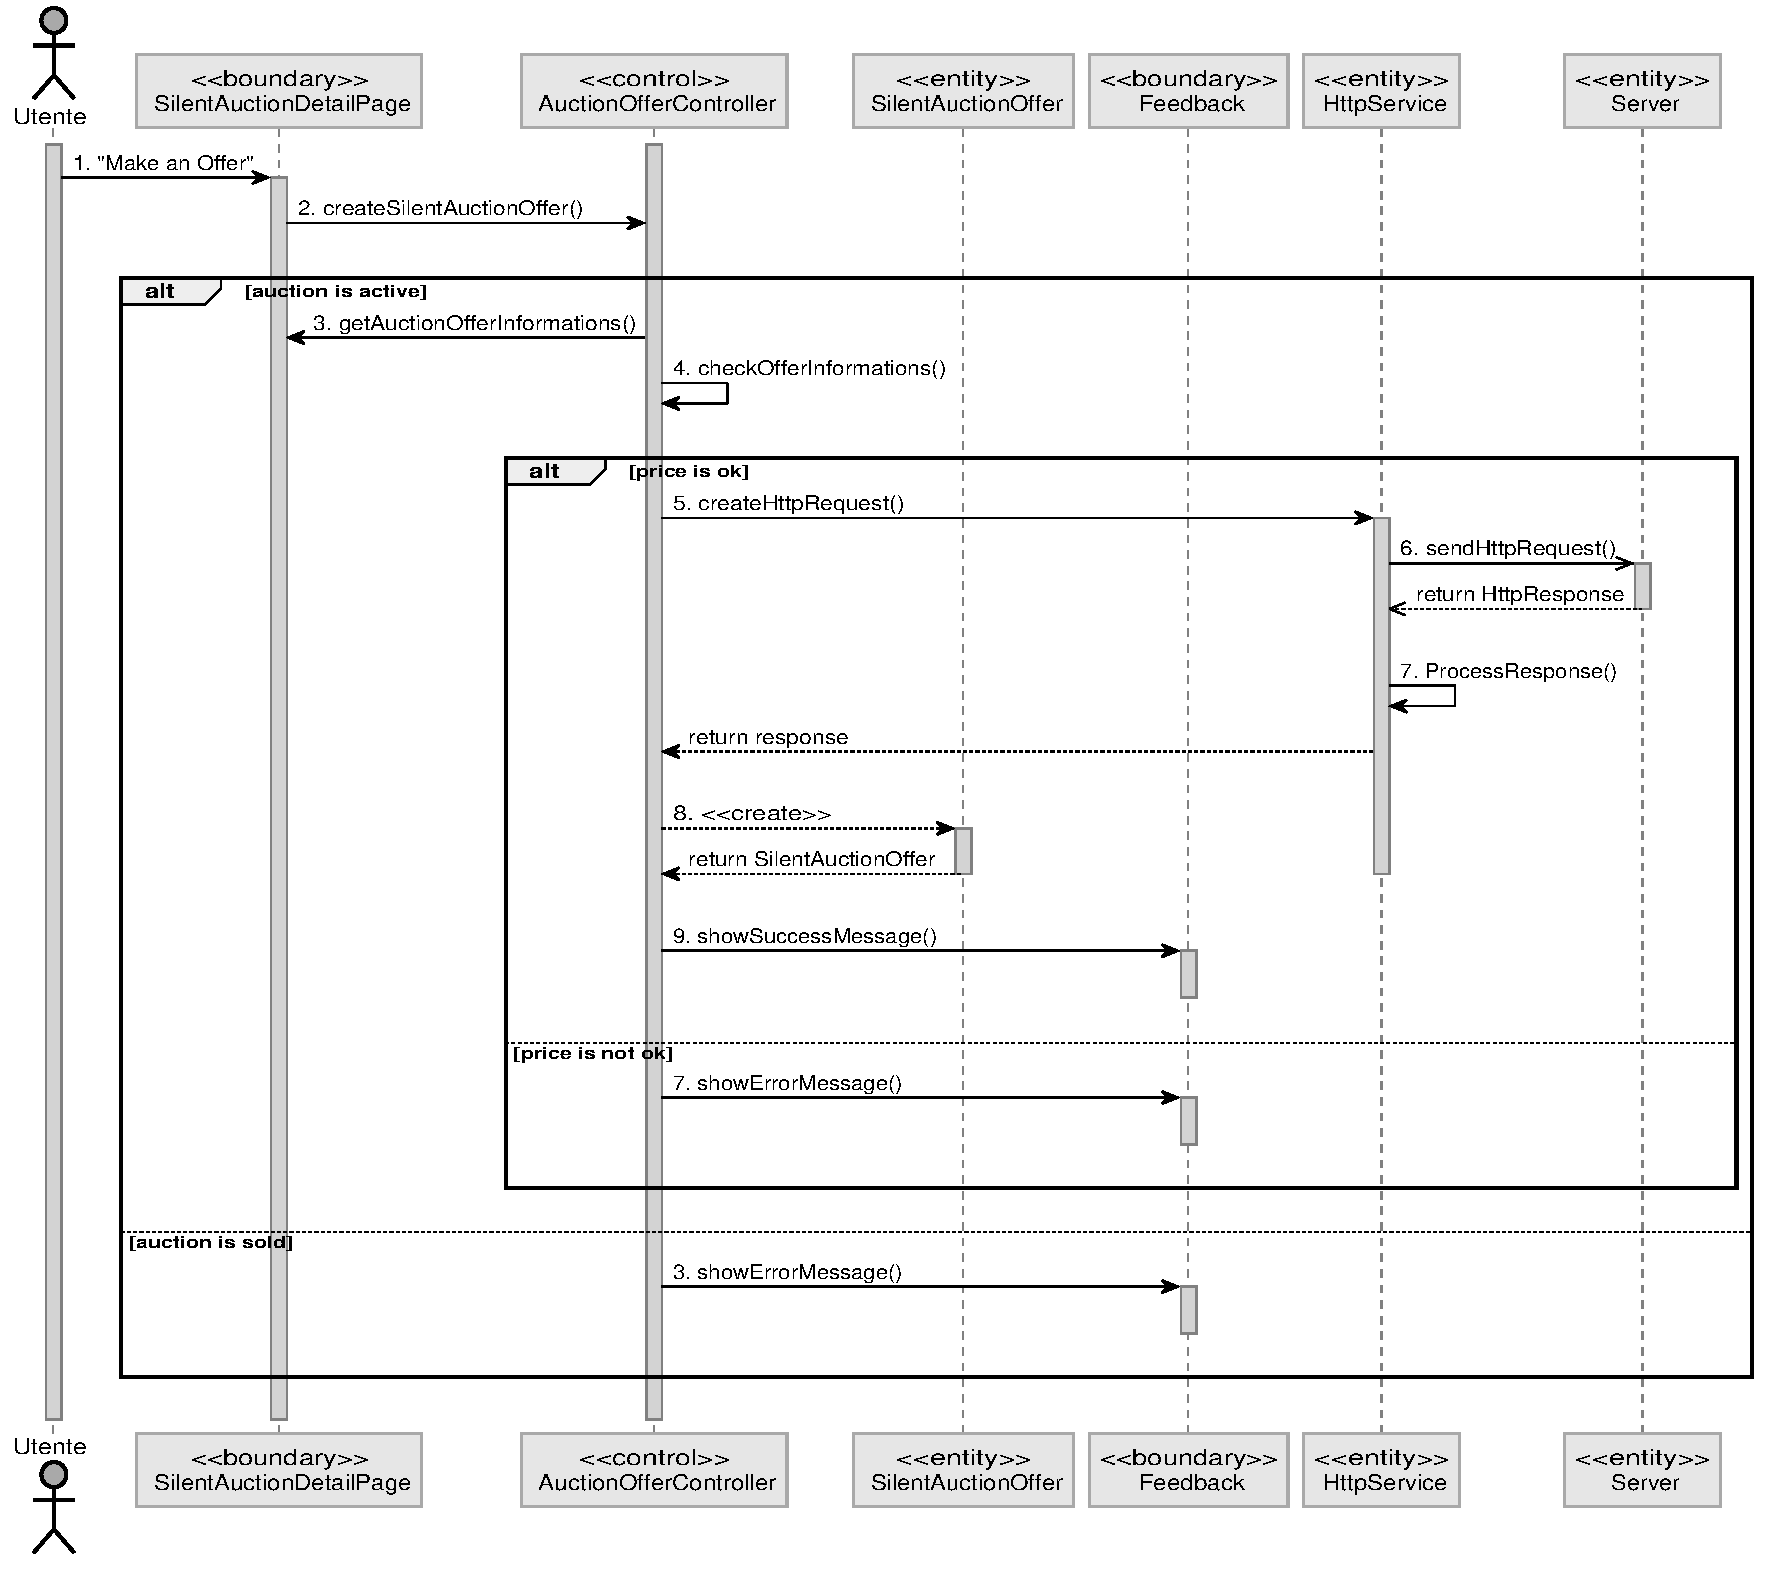
\includegraphics[width=\textwidth]{assets/sequence/piazzare_offerta_asta_silenziosa.pdf}

\pagebreak
\subsection{Caso d'uso: Aggiunta Link Social}
Il seguente Sequence Diagram descrive il processo di aggiunta di un nuovo link social all'interno della pagina profilo dell'utente.\\ 
Il sistema prende, in generale, tutti i valori presenti nel form, e verifica che siano corretti. A questo punto invia una richiesta al server e restituisce un risultato. Nel caso l'esito sia positivo, aggiorna il model correttamente e notifica l'utente.\bskip
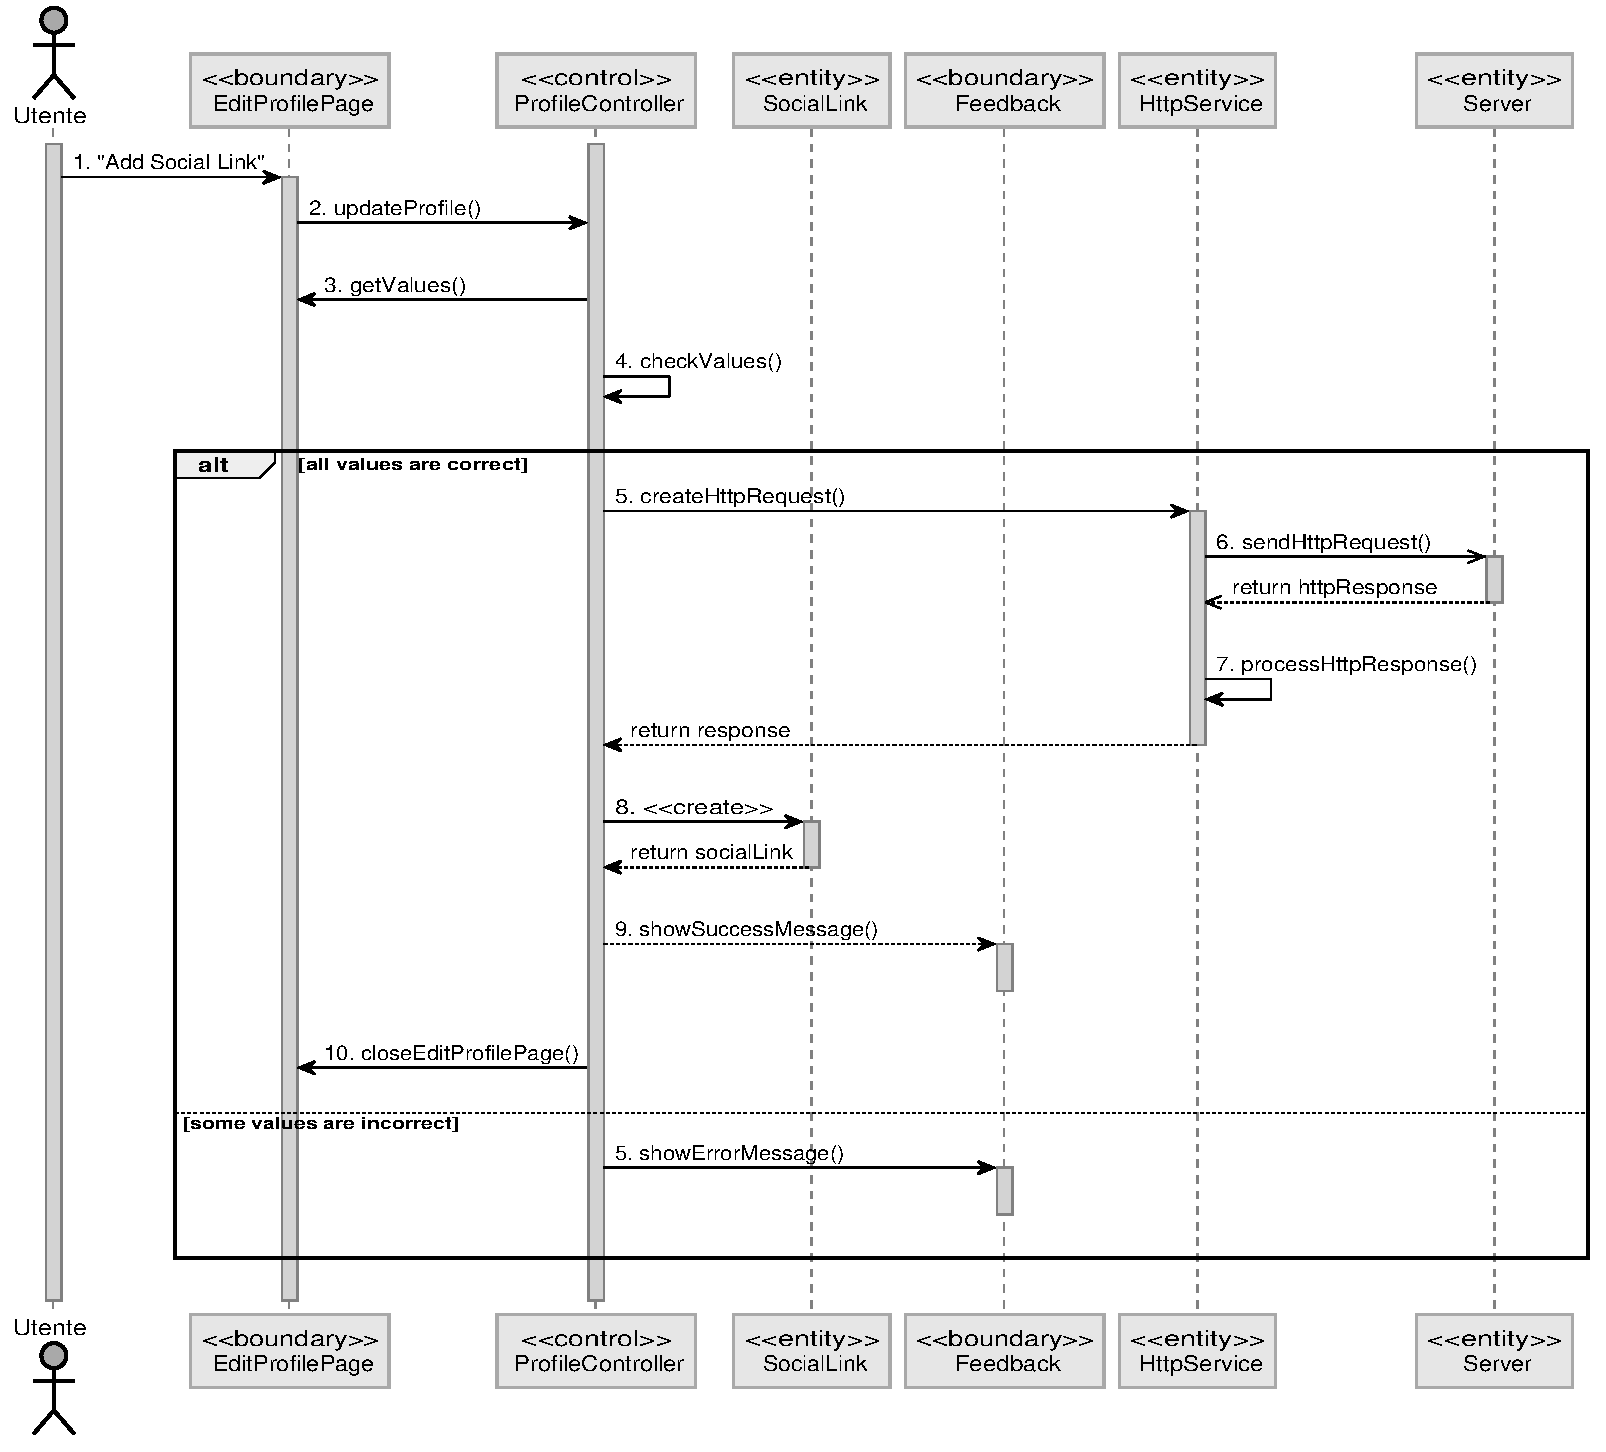
\includegraphics[width=\textwidth]{assets/sequence/aggiungere_link_social.pdf}

\pagebreak
\subsection{Caso d'uso: Storico Aste create}
Il seguente Sequence Diagram descrive il processo per cui l'utente visualizza lo storico delle aste create. 
Analogamente ai sequence mostrati in precedenza, l'utente naviga all'interno della schermata e il sistema invia una richiesta al server che restituirà le aste create all'utente.\bskip
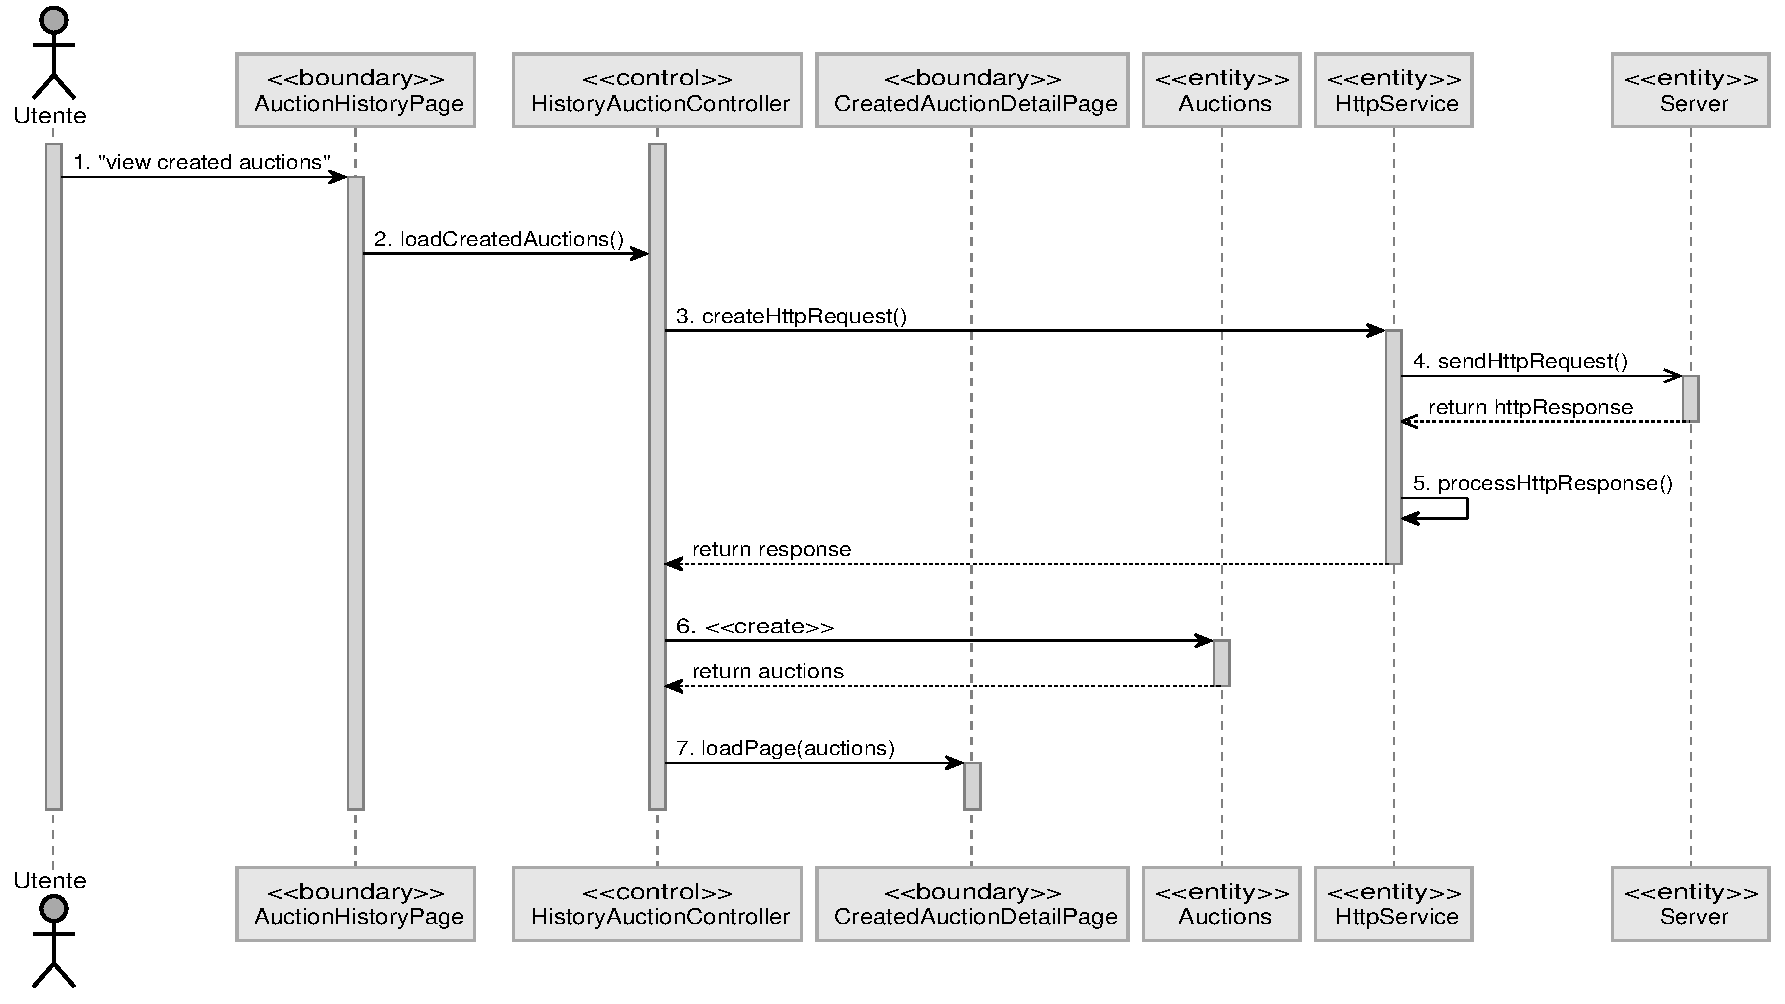
\includegraphics[width=\textwidth]{assets/sequence/visualizzazione_storico_aste_ancora_attive.pdf}
